\documentclass[10pt,journal,a4paper]{IEEEtran}
\usepackage[T1]{fontenc}
\usepackage{graphicx}
\usepackage{booktabs}
\usepackage{amsmath}
\usepackage{amssymb}
\usepackage{url}
\urlstyle{same}
\usepackage[hidelinks]{hyperref}

\begin{document}

\title{\vspace{-1.6em}\footnotesize\textsc{The University of Lahore $\bullet$ Department of Intelligent Systems $\bullet$ AI-101}\\[0.9em]
\Large Task B1: Detecting Fraudulent Job Postings}

\author{\normalsize Manaal Pervaiz \quad$\vert$\quad Roll No. 70173809 \quad$\vert$\quad Section BSES A\\
\normalsize Repository: \url{https://github.com/manaal6/AI101-ML-Assignment-70173809}\\
\normalsize Instructor: Dr. Muhammad Awais, AI Architect}
\date{}
\maketitle

\section{Introduction}
Job boards carry advertisements from real employers and from scammers who
promise non-existent jobs, harvest personal data or ask for fees. Only 4.84\% of
the 17,880 EMSCAD postings are fraudulent, but each reaches many applicants, so
a platform must triage them automatically. The record mixes free text with
structured metadata: a missing company profile is suspicious, and phrases such
as ``data entry'' or ``earn'' recur in scams. We compare Logistic Regression, a
Linear SVM and LightGBM on the same representation. LightGBM was best on
validation PR-AUC (0.954); on test it reached PR-AUC 0.919 and F1 0.831. Text
carries most of the signal, metadata adds 0.029 PR-AUC, and class weighting
raises validation F1 from 0.809 to 0.848.

\section{Problem Statement}
Each posting is a pair $x=(x_{\text{struct}}, x_{\text{text}})$, where
$x_{\text{struct}}$ holds 16 structured attributes and $x_{\text{text}}$ is the
concatenation of five free-text fields. The label is $y \in \{0,1\}$, with
$y=1$ fraudulent. The task is supervised binary classification with severe
imbalance (4.84\% positive). Success is measured by F1 on the fraud class and
by PR-AUC, with ROC-AUC reported for completeness; accuracy is not a selection
criterion because a constant ``real'' prediction already scores about 95\%.

\section{Dataset Used}
The Real or Fake Job Posting Prediction dataset \cite{bhardwaj} is the EMSCAD
corpus from the University of the Aegean, distributed on Kaggle and licensed
CC0 (verified through the Kaggle API). It has 17,880 rows and 18 columns: one
identifier, the target, five text fields (title, company profile, description,
requirements, benefits), three binary flags (telecommuting, company logo,
screening questions) and eight metadata columns.

Cleaning removes no rows. The identifier is dropped; the five text fields are
HTML-unescaped, lower-cased and stripped of tags, URLs, e-mail addresses,
punctuation and digits, then concatenated. Country is derived from the first
token of \texttt{location} (\texttt{US, NY, New York} $\rightarrow$ US) because
the raw field has 3,105 values. \texttt{department} is dropped (64.6\% missing,
1,337 values). Missingness is preserved as signal with indicators for company
profile, requirements and benefits, plus a salary-present flag.

\section{Dataset Statistics}
Table~\ref{tab:stats} summarises the data. Figure~\ref{fig:rates} shows two
required EDA splits. A posting without a company logo is fraudulent 15.93\% of
the time versus 1.99\% with a logo; part-time postings are fraudulent 9.28\% of
the time and temporary ones 0.83\%. The strongest single signal is a missing
company profile: 17.74\% fraud versus 1.91\%.

\section{Methodology}
\subsection{Learning Setting}
Three classifiers share one representation: Logistic Regression as a linear
baseline whose coefficients expose fraud-indicative terms; a Linear SVM, which
suits sparse high-dimensional text; and LightGBM, which captures interactions
between text and structured features. The \texttt{ColumnTransformer}
median-imputes and standardises the 7 numeric features, passes the 3 binary
flags, one-hot encodes the 6 categoricals (rare levels below 0.5\% grouped), and
applies TF-IDF to the text (word 1--2 grams, 20,000 features,
\texttt{min\_df}=3, sublinear term frequency). The design matrix has 20,102
columns. Imputers, encoder and vectoriser are fitted on the training split only.

\subsection{Data Split Approach}
A stratified 70/15/15 split with seed 42 gives 12,516 training, 2,682
validation and 2,682 test postings, with 606/130/130 frauds. Logistic
Regression and the SVM are tuned by 3-fold stratified cross-validation on the
training split; validation chooses every threshold and the best model, and test
is evaluated once. The TF-IDF vocabulary is fixed on the training split and
reused by the CV folds, which is mildly optimistic; no validation or test text
influences it.

\begin{table}[t]
\centering
\caption{Dataset statistics and split.}
\label{tab:stats}
\footnotesize
\setlength{\tabcolsep}{3pt}
\begin{tabular}{@{}ll@{}}
\toprule
Property & Value \\
\midrule
Samples (rows $\times$ columns) & 17,880 $\times$ 18 \\
Inputs & 7 numeric, 3 binary, 6 categorical, 1 text \\
Fraudulent / real & 866 (4.84\%) / 17,014 \\
Missing values & salary 84.0\%, dept.\ 64.6\%, profile 18.5\% \\
Description length & 1,218 chars, 170 words (mean) \\
Duplicate rows & 0 \\
Train / validation / test & 12,516 / 2,682 / 2,682 \\
Fraud in each split & 606 / 130 / 130 \\
Design matrix & 20,102 columns after TF-IDF \\
\bottomrule
\end{tabular}
\end{table}

\begin{figure}[t]
\centering
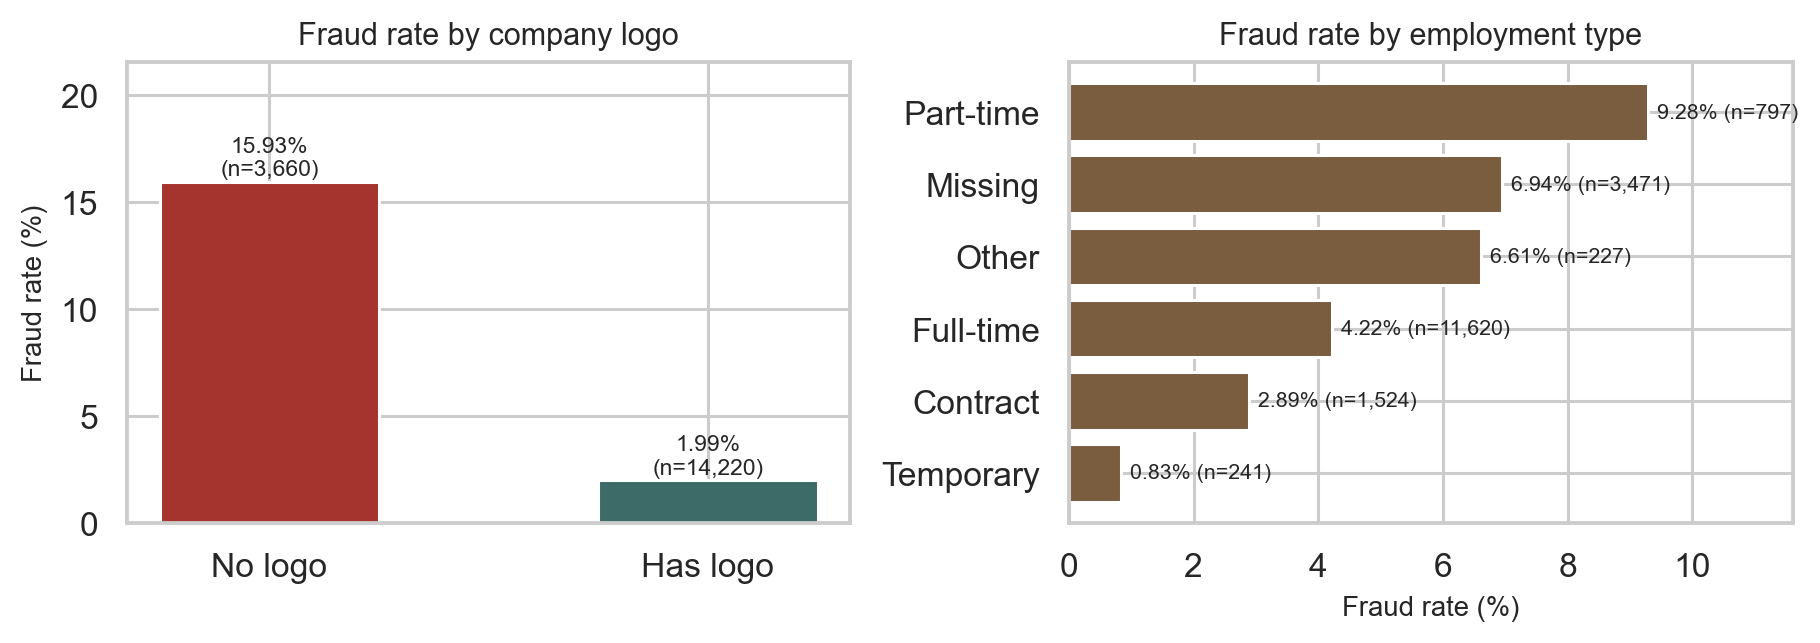
\includegraphics[width=0.92\columnwidth]{../figures/fig3_fraud_rates.png}
\caption{Fraud rate by company logo and by employment type (all 17,880
postings).}
\label{fig:rates}
\end{figure}

\subsection{Parameter Settings}
Table~\ref{tab:params} lists the search and the selected values. LightGBM uses a
fixed sparse configuration because a 150-tree fit costs about a minute on the
available CPU; its values are listed in the table. Thresholds are chosen on the
validation split to maximise fraud F1: 0.753 for Logistic Regression, 0.417 for
the SVM and 0.529 for LightGBM.

\begin{table}[t]
\centering
\caption{Hyperparameter settings and selected values.}
\label{tab:params}
\footnotesize
\setlength{\tabcolsep}{2.5pt}
\begin{tabular}{@{}l p{3.8cm} l@{}}
\toprule
Model & Search space & Selected \\
\midrule
Logistic reg. & $C \in \{0.1,1\}$ & $C=1$ \\
Linear SVM & $C \in \{0.01,0.1\}$ & $C=0.1$ \\
LightGBM & 150 trees, 31 leaves, lr 0.1,\newline spw 19.65, ff 0.3 & fixed \\
\bottomrule
\end{tabular}
\end{table}

\section{Results and Analysis}
\subsection{Results}
Table~\ref{tab:test} reports the test set. LightGBM has the best PR-AUC
(0.919) and the highest validation PR-AUC (0.954), so it is the selected model;
the SVM has a slightly higher test F1 (0.836 versus 0.831), a difference of one
posting. At its threshold LightGBM produces 2,540 true negatives, 12 false
positives, 29 false negatives and 101 true positives.

\begin{table}[t]
\centering
\caption{Test-set results (2,682 postings, 130 fraudulent). Best per column in bold.}
\label{tab:test}
\footnotesize
\setlength{\tabcolsep}{3pt}
\begin{tabular}{@{}lcccccc@{}}
\toprule
Model & Thr. & Prec. & Recall & F1 & PR-AUC & ROC-AUC \\
\midrule
Logistic Reg. & 0.753 & 0.811 & \textbf{0.823} & 0.817 & 0.903 & 0.991 \\
Linear SVM & 0.417 & \textbf{0.895} & 0.785 & \textbf{0.836} & 0.918 & 0.991 \\
LightGBM & 0.529 & 0.894 & 0.777 & 0.831 & \textbf{0.919} & \textbf{0.992} \\
\bottomrule
\end{tabular}
\end{table}

\begin{figure}[t]
\centering
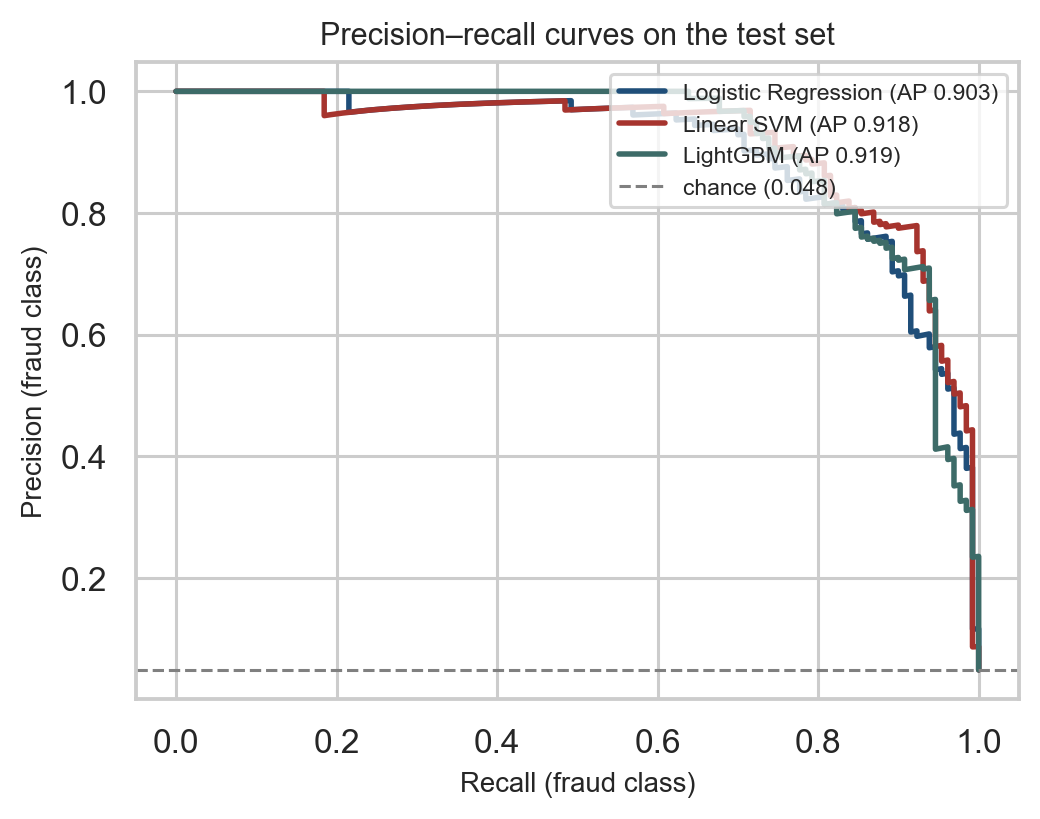
\includegraphics[width=0.74\columnwidth]{../figures/fig4_precision_recall_curves.png}
\caption{Precision--recall curves on the test set; average precision is 0.903
(Logistic Regression), 0.918 (SVM) and 0.919 (LightGBM).}
\label{fig:pr}
\end{figure}

\subsection{Analysis}
\paragraph{Why accuracy misleads}
A model that always predicts ``real'' scores 0.9515 and catches none of the 130
frauds. LightGBM reaches 0.9847, a gap of only 3.3 points, yet F1 is 0.831 and
it misses 29 fraudulent postings. The confusion matrix, not accuracy, shows the
cost: 12 legitimate employers are blocked and 29 scams pass. F1 and PR-AUC are
the right metrics because they weight the rare class.

\paragraph{Text versus structured features}
The mandatory ablation (Table~\ref{tab:ablation}) shows that text carries most
of the signal. Structured metadata alone reaches PR-AUC 0.795 and F1 0.698;
text alone reaches 0.890 and 0.837. Combining them raises PR-AUC by 0.029 over
text alone and by 0.124 over structured alone, but F1 moves by $-0.006$ versus
text alone. The honest reading is that metadata improves ranking (PR-AUC) while
the threshold-based F1 stays flat: the extra information reorders postings near
the boundary rather than adding many new true positives.

\begin{table}[t]
\centering
\caption{Ablation with LightGBM on the test set. Best per column in bold.}
\label{tab:ablation}
\footnotesize
\setlength{\tabcolsep}{3pt}
\begin{tabular}{@{}lcccc@{}}
\toprule
Features & PR-AUC & Precision & Recall & F1 \\
\midrule
Structured only & 0.795 & 0.794 & 0.623 & 0.698 \\
Text only & 0.890 & 0.888 & \textbf{0.792} & \textbf{0.837} \\
Combined & \textbf{0.919} & \textbf{0.894} & 0.777 & 0.831 \\
\bottomrule
\end{tabular}
\end{table}

\paragraph{Indicative words and structured features}
The fraud-leaning terms are \emph{aptitude staffing} (2.61), \emph{accion}
(2.59), \emph{earn} (2.36), \emph{hotel} (2.20), \emph{aptitude} (2.15),
\emph{money} (2.14), \emph{link} (2.10) and \emph{data entry} (2.00). Several
are company names or boilerplate from repeated scam templates rather than
semantic cues. The most fraud-leaning structured
features are industry \emph{Oil \& Energy} (2.14), country AU (1.57), missing
country (1.57), industry \emph{Accounting} (1.56) and function
\emph{Administrative} (1.31); a company logo is the strongest real-leaning
feature ($-1.13$). The missing-profile indicator is positive ($+0.27$), much
smaller than its univariate effect because it correlates with the logo flag;
the two together describe the same company-quality signal.

\paragraph{False positives}
Only 12 of 2,552 real test postings are flagged. The highest-scoring is a
``Receptionist'' posting (0.894) with no company profile, no logo and a US
location; next are a ``Sr Customer Care Executive'' (0.841, India) and a ``Land
Surveying Field Crew Chief'' (0.838, US). All three are ordinary small-employer
advertisements that look like scams on the metadata the model trusts --- the
expected failure mode of a metadata-driven detector, and the argument for human
review.

\paragraph{Class weighting and limitations}
Balancing the classes raises validation PR-AUC from 0.8786 to 0.9199 and
validation F1 from 0.8085 to 0.8482, at the cost of precision. The test set has
130 frauds, so one posting moves recall by 0.8 points, and LightGBM's validation
F1 (0.901) overstates its test F1 (0.831), a warning against trusting a single
split. Country is inferred from free-text location, and the corpus has no
timestamp, so drift cannot be measured; probabilities were not calibrated.

\section{Conclusion}
A combined TF-IDF and metadata model detects 78\% of fraudulent postings at 89\%
precision (F1 0.831, PR-AUC 0.919); text carries most of the signal. Metadata
adds ranking quality rather than recall, and class weighting is essential at
4.84\% prevalence. Next: calibration and temporal validation.

\section*{AI Use Disclosure}
I used opencode, an AI coding assistant, for notebook scaffolding, plotting code
and a first draft of this report's LaTeX, which I edited. I verified every
number against the executed notebook outputs, re-ran the notebook top to bottom,
and checked the leakage controls myself. I take full responsibility for this
work.

\begin{thebibliography}{1}
\raggedright
\bibitem{bhardwaj} S.~Bhardwaj, ``Real or Fake Job Posting Prediction,''
Kaggle, 2020. \url{https://www.kaggle.com/datasets/shivamb/real-or-fake-fake-jobposting-prediction}.

\bibitem{sklearn} F.~Pedregosa \emph{et al.}, ``Scikit-learn: Machine learning
in Python,'' \emph{Journal of Machine Learning Research}, vol.~12,
pp.~2825--2830, 2011.

\bibitem{lgbm} G.~Ke \emph{et al.}, ``LightGBM: A highly efficient gradient
boosting decision tree,'' \emph{Advances in Neural Information Processing
Systems}, vol.~30, 2017.
\end{thebibliography}

\end{document}
